\documentclass[a4paper, 14pt]{article}

% T2A for cyrillic
\usepackage{soul}

\usepackage[utf8]{inputenc}
\usepackage[T2A]{fontenc}
\usepackage[ukrainian]{babel}
\usepackage{tempora}

% package to change sections appearance
\usepackage{titlesec}
% package for lists
\usepackage{enumitem}
% reduce space before list
\setlist{nolistsep}
% package for inserting images
\usepackage{graphicx}
% package for hyperlinks
\usepackage[colorlinks=true]{hyperref}


% lists geometry
\let\olditemize\itemize
\renewcommand{\itemize}{
  \olditemize
  \setlength{\itemsep}{-8pt}
  \setlength{\parskip}{-8pt}
  \setlength{\parsep}{-8pt}
}

% line spacing
\usepackage{setspace}
\onehalfspacing

% margins
\usepackage[total={5.4in, 8.7in}]{geometry}

% this is a global declaration that changes the appearance of the section command
\titleformat{\section}{\large\scshape\raggedright}{}{0em}{}
% this is a global declaration that changes the appearance of the subsection command
\titleformat{\subsection}{\tt\raggedright}{}{0em}{}

\begin{document}
\begin{center}
  \textsc{\Huge{\so{Іван Сергієнко}}}
\end{center}

% photo (optional)
\begin{center}
  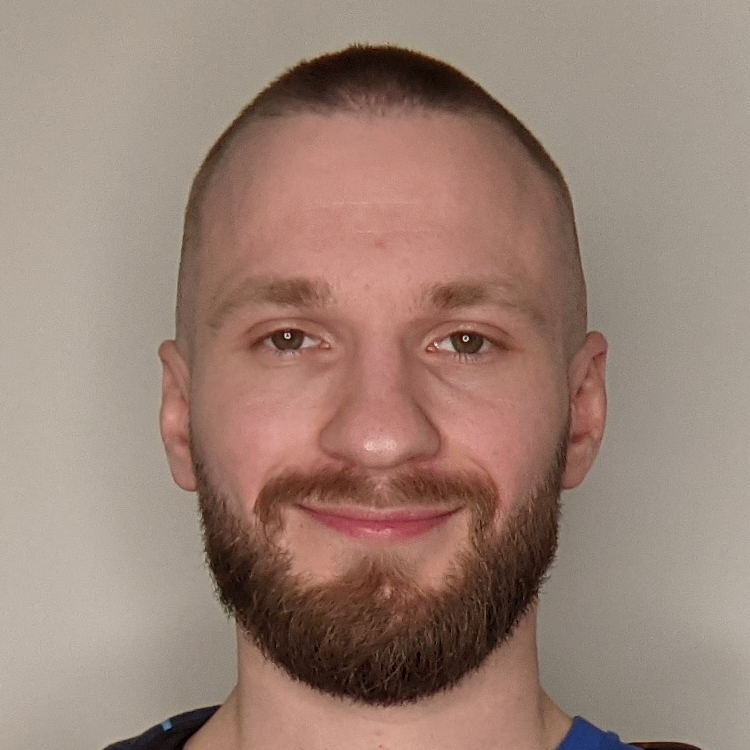
\includegraphics[width=50mm]{ava-2021.png}
\end{center}

\section{Навички}
  \begin{itemize}
    \item Пайка (THT) - спаяв штук 20 плат як хоббі  \\
    \item Користування мультиметром \\
    \item Базові знання електроніки та схемотехніки \\
    \item З осцилографом працював один раз в університеті :) \\
    \item Вміння читати документацію, в т.ч. англійською \\ 
    \item Прошивка - AVR Atmel, Arduino, ESP8266 \\
    \item Базове програмування на С для мікроконтролерів \\
    \item Базове програмування на Python - класичний machine learning, навчання нейромереж \\
    \item Базове користування Linux, bash \\
    \item Програмування на JavaScript - 10 років досвіду
  \end{itemize}

  \subsection{Статті}
    \begin{itemize}
      \item Синтезування синусоїдальної звукової хвилі за допомогою JavaScript: \url{https://medium.com/@darthvanger/synthesize-sound-with-javascript-sine-wave-940f9cd7dae2}
    \end{itemize}

\section{Освіта}
  НТУУ ``КПІ'' - неповна вища
  \begin{itemize}
    \item Прикладна фізика - 3 роки \\
    \item Поліграфія - 3 роки
  \end{itemize}

  \subsection{Курси}
  \begin{itemize}
    \item Історія, технологія та безпека Інтернету - Університет Мічігану (Coursera) \\
    \item Основи алгоритмів (школа Projector) \\
    \item Машинне навчання (Hillel IT school) \\
    \item Технологія Біткоіну та криповалют - Уніврситет Прінстону (Coursera) \\
    \item Розробка веб-застосунків на Java (EPAM)
  \end{itemize}

\section{Володіння мовами}
	English - Upper Intermediate (десь 8/10, розмовна і письмова). \\
  Я працював 2 роки в британській команді (онлайн) - розмовляв англійською кожен день

\section{Контакти}
	tel. +380930780138 (telegram, whatsapp, viber) \\
	email: darthvanger@gmail.com \\
  linkedin: \url{https://www.linkedin.com/in/ivan-sergiienko-76494b73}

\section{Персональна інформація}
	Вік: 35 років \\
  Місце проживання: м. Київ, правий берег

\section{Досвід роботи}
  \subsection{Jan 2024 - Aug 2026: розробник програмного забезпечення - Innovecs}
  Розробка слот ігор для різних замовників (Болгарія, Англія), а також онлайн покер.

  \subsection{Sep 2022 - Jan 2024: розробник програмного забезпечення - FreedomFi}

  Розробка інтерфейсу для 5G роутеру та блокчейну.

  \subsection{Jan 2022 - Sep 2022: перерва в кар'єрі}

  \subsection{Feb 2016 - Dec 2021: розробник програмного забезпечення - DataArt}  
  Розробка систем для мереж супермаркетів для клієнту з Англії.
  \begin{itemize}
    \item Розробка системи менеджменту автопарку \\
    \item Розробка системи менеджменту поставок \\
    \item Розробка системи менеджменту кандидатів на вакансії
  \end{itemize}

  \subsection{Sep 2014 - Jan 2016: розробник програмного забезпечення - ISD Group}
  Підтримка та розробка соціальної мережі SvitMam.

  \subsection{May 2010 - Sep 2010: офіціант на банкетах - Moody Gardens (Техас, США)}

\end{document}
